\documentclass[10pt,a4paper]{article}
\usepackage[utf8x]{inputenc}
\usepackage{ucs}
\usepackage{amsmath}
\usepackage{amsfonts}
\usepackage{amssymb}
\usepackage{a4wide}
\usepackage{comment}
\usepackage[pdftex]{graphicx}
\usepackage{epstopdf}
\newcommand{\cmd}[1]{\texttt{#1}}
\newcommand{\remove}{}
\newcommand{\dir}[1]{\textsf{#1}}
\newcommand{\pop}{Depiler\xspace}
\newcommand{\push}{Empiler\xspace}
\newcommand{\tete}{LireTete}
\newcommand{\sommet}{LireSommet}
\newcommand{\empt}{EstVide}
\newcommand{\enqueue}{Enfiler\xspace}
\newcommand{\dequeue}{Defiler\xspace}
\newcommand{\get}{\ensuremath{\leftarrow\ }}
\usepackage{enumitem}
\usepackage{pifont}


\usepackage{comment}
\usepackage{algorithm}
\usepackage[noend]{algpseudocode}
\usepackage{tcolorbox}

\newtcolorbox{mybox}[3][]
{
  colframe = #2!25,
  colback  = #2!10,
  coltitle = #2!20!black,  
  title    = {#3},
  #1,
}
\newcommand*\Let[2]{\State #1 $\gets$ #2}


\excludecomment{solution}
\includecomment{solution}

\title{IF223 - Algorithmique Distribuée - TD3}
\date{1 Avril 2022}
\author{Rohan Fossé}
\date{\texttt{rfosse@labri.fr}}


\begin{document}
\maketitle


\section*{Exercice 1}

On considère l’Algorithme vu en cours. Cet algorithme construit un arbre couvrant (\textit{spanning tree} en anglais), étant donnée la racine de l’arbre. On considère un système distribué représenté par le graphe en Figure 1, où chaque processus a un identifiant unique dans l’ensemble \{a, b, $\ldots$ f \} et le processus a est la racine de l’arbre à construire, c’est-à-dire pr = a dans le pseudo-code.

\begin{figure}[h!]
    \centering
    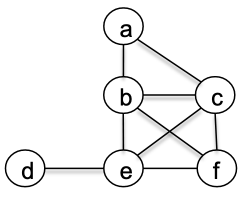
\includegraphics[scale=0.6]{fig1.png}
    \caption{Figure 1}
    \label{fig:fig1}
\end{figure}

\begin{enumerate}
    \item Donner deux arbres couvrants différents enracinés en $a$ pour le graphe en Figure 1.
    \item On suppose que le système est synchrone. Donner une exécution de l'algorithme et montrer l'arbre couvrant généré par cette exécution. Est-il possible de construire un autre arbre couvrant enraciné en $a$ en exécutant le même algorithme sur le même graphe ?
    \item On considère maintenant un système asynchrone. Est-il possible que deux exécutions différentes construisent deux arbres couvrants différents ? Si oui, donnez ces exécutions en forme de suite de graphes.
    \item On considère les exécutions admissibles pour le modèle asynchrone. pourquoi tout processus aura un et un seul parent ?\\
    Pourquoi ce n'est pas possible qu'un cycle soit crée?
\end{enumerate}

\newpage

\section*{Exercice 2}

On considère l'algorithme en Figure 2. Quel problème résout cet algorithme ? Expliquer en français le fonctionnement de l'algorithme. Il y a un processus $p_r$ désigné avant l'exécution. Les valeurs initiales pour les variables locales à un processus $p_i$ pour tout $i \in \{0, \ldots, n-1 \}$ sont :
\begin{itemize}
    \item parent = $\bot$
    \item children = $\emptyset$
    \item unexplored = tout les voisins de $p_i$
\end{itemize}


\begin{figure}[h!]
    \centering
    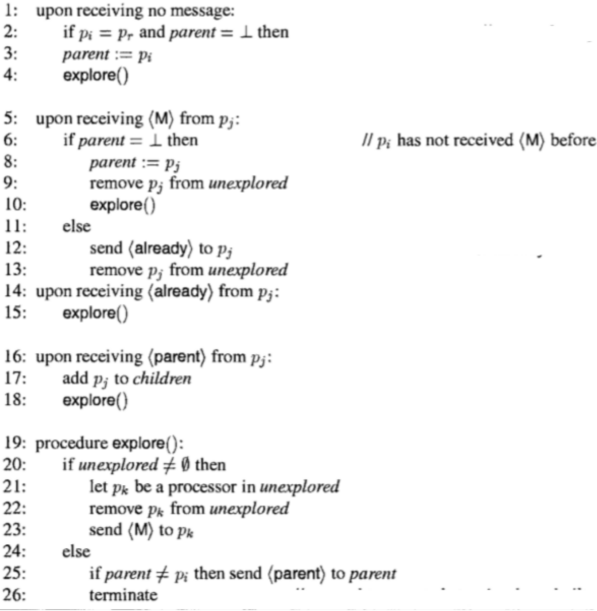
\includegraphics[scale=0.6]{fig2.png}
    \caption{Algorithme mystère: pseudo-code pour le processus $p_i$}
    \label{fig:my_label}
\end{figure}

\section*{Exercice 3}

On considère le système distribué en Figure 3. En supposant que le système est synchrone,
donner une exécution de l’algorithme pour l’élection d’un leader avec complexité $\Omega(n logn)$ où n est le nombre
de processus dans le système. Expliquer le rôle des informations insérées dans les messages $<$ probe, j, k, d $>$ et $<$ reply, j, k $>$.

\begin{figure}[h!]
    \centering
    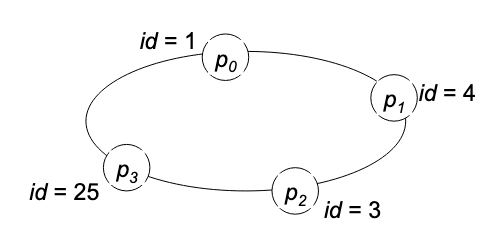
\includegraphics{fig3.png}
    \label{fig:my_label}
\end{figure}

\section*{Exercice 4}

On considère un anneau anonyme de n processus où chaque processus a une entrée 1 ou 0.
Tous les processus doivent retourner 0 s’il existe un processus dont le bit d’entrée est 0, sinon ils doivent
retourner 1.
\begin{itemize}
    \item Concevoir un algorithme non uniforme asynchrone qui résout le problème avec une complexité en
message en O(n2).
    \item Concevoir un algorithme non uniforme synchrone qui résout le problème avec une complexité en
message en O(n).
\end{itemize}

\end{document}





